\documentclass[xcolor={usenames,dvipsnames}]{beamer}
\usepackage[utf8]{inputenc}
\usepackage[english]{babel}

% -- Including some standard packages --
\usepackage{graphicx}
\usepackage{soul}
\usepackage{hyperref}
\usepackage{colortbl}
\usepackage{dsfont}
\usepackage{soul}

% -- Choosing theme --

\usetheme{Boadilla}
\usecolortheme{whale}
% \usefonttheme[onlymath]{serif}

% Tikz
\usepackage{tikz}
\usetikzlibrary{matrix,positioning,fit,backgrounds,intersections}

% -- Cross signs --
\usepackage{pifont}% http://ctan.org/pkg/pifont
\newcommand{\cmark}{\ding{51}}%
\newcommand{\xmark}{\ding{55}}%
\newcommand{\xopt}{\ding{48}}%

% -- Custom commands --
\DeclareMathOperator*{\argmax}{arg\,max}
\DeclareMathOperator*{\argmin}{arg\,min}

\title[Elliptic Curves]{\textbf{Elliptic Curve Optimizations. EC Pairing.}}
\author{Distributed Lab\vspace{-2em}}
\date{May 16, 2024}

\titlegraphic{
    \includegraphics[width=0.9\textwidth]{images/pairing.png}
}

\expandafter\def\expandafter\insertshorttitle\expandafter{%
  \insertshorttitle\hfill%
  \insertframenumber\,/\,\inserttotalframenumber}

\AtBeginSection[]{
  \begin{frame}
  \vfill
  \centering
  \begin{beamercolorbox}[sep=8pt,center,shadow=true,rounded=true]{title}
    \usebeamerfont{title}\insertsectionhead\par%
  \end{beamercolorbox}
  \vfill
  \end{frame}
}

\begin{document}
	\frame {
		\titlepage
	}
 
	\begin{frame}{Plan}
        \tableofcontents
    \end{frame}

	\section{Preliminaries}
    \begin{frame}{Field}
        \begin{definition}{}
            \textbf{Field} $K$ is a set equipped with appropriate \textbf{addition} and \textbf{multiplication} operations with the corresponding well-defined inverses, where you can perform the basic arithmetic.
        \end{definition}
        \pause
        \begin{exampleblock}{}
            \begin{itemize}
                \item $\mathbb{R}$ (real numbers) is a field.\pause
                \item $\mathbb{Q}$ (rational numbers) is a field.\pause
                \item $\mathbb{C}$ (complex numbers) is a field.\pause
                \item $\mathbb{N}$ (natural numbers) is not a field: there is no additive inverse for $2$ ($-2$ is not in $\mathbb{N}$).\pause
                \item $\mathbb{Z}$ (integers) is not a field: additive inverse is defined, but the multiplicative is not ($2^{-1}$ is not defined).
            \end{itemize}
        \end{exampleblock}
    \end{frame}
 
	\begin{frame}{Finite Field}	
		\begin{definition}{}
		    \textbf{Finite field} $\mathbb{F}_p$ is a set $\{0,1,\dots,p-1\}$ equipped with basic arithmetic ($+$ and $\times$) modulo $p$.
		\end{definition}
        \pause
        \begin{example}
            $\mathbb{F}_5$ is a set with elements $\{0,1,2,3,4\}$. Examples of calculations:
            \begin{enumerate}
                \item $3 + 4 = 7 = 2$ (in $\mathbb{F}_5$);
                \item $3 - 4 = -1 = 4$ (in $\mathbb{F}_5$);
                \item $3 \times 4 = 12 = 2$ (in $\mathbb{F}_5$);
                \item $3^{-1} = 2$ (since $3 \cdot 2 = 1$ in $\mathbb{F}_5$);
                \item $2/3 = 2 \times 3^{-1} = 4$ in $\mathbb{F}_5$.
            \end{enumerate}
        \end{example}

        Typically, $p$ is a large (e.g., 254-bit) \textbf{prime number}.
	\end{frame}

    \begin{frame}{Finite Field Illustration}
        \begin{figure}
            \centering
            \includegraphics[width=\textwidth]{images/clock_f12.png}
            \caption{Illustration of performing addition in $\mathbb{Z}_{12}$ (not really a field, but the rules are identical besides inversion).}
        \end{figure}
    \end{frame}

    \begin{frame}{Elliptic Curve}	
        \begin{definition}
            \textbf{Elliptic Curve} $E(K)$ in short \textit{Weierstraß form} over the field $K$ is a set of coordinates $(x,y)$ from $K$ such that
            \begin{equation*}
                y^2 = x^3 + ax + b, \;\;\; (a,b \in K)
            \end{equation*}
            together with a ``point at infinity'' $\mathcal{O}$.
        \end{definition}
        \pause
        \textbf{BN254} (or \textbf{BN256}/\textbf{BN128}) is the curve over $K=\mathbb{F}_p$ where:
        \begin{gather*}
            y^2 = x^3 + 3 \;\;\;\;\; (a=0,b=3) \\
            p = \mathsf{0x30644e72e131a029b85045b68181585d97...}\\{...816a916871ca8d3c208c16d87cfd47}
        \end{gather*}
    \end{frame}

    \begin{frame}{Elliptic Curve on the Figure}	
        \begin{figure}
            \centering
            \includegraphics[width=\textwidth]{images/curves.png}
            \caption{Illustration of various elliptic curves over $\mathbb{R}$ (that is, $E(\mathbb{R})$).}
        \end{figure}
    \end{frame}

    \begin{frame}{Actually, these are Elliptic Curves...}	
        But actual elliptic curves look more like that...
    
        \begin{figure}
            \centering
            \includegraphics[width=0.65\textwidth]{images/actual_ec.png}
            \caption{Illustration of an elliptic curve $E(\mathbb{F}_{11}): y^2 = x^3 - 2x$.}
        \end{figure}
    \end{frame}
    
    \begin{frame}{Group structure}	
        \begin{definition}
            \textbf{Group} $(\mathbb{G}, \oplus)$ is just a set with defined operation $\oplus$, which has ``nice'' properties (e.g., closure).
        \end{definition}
        \pause
        \textbf{Idea:} A set of objects is useless unless we have practical relations between elements. For example, $7$ and $13$ are integers, but the structure is worthless without the ability to add/multiply them.
        \pause
        \begin{theorem}
            $(E(\mathbb{F}_p), \oplus)$ is a group where operation $\oplus$ between points $P,Q \in E(\mathbb{F}_p)$ means drawing a line between $P$ and $Q$ (or tangent line if $P=Q$), finding intersection with $E(\mathbb{F}_p)$ and ``reflecting around $Ox$ axis'' (negating $y$ component). We denote the group order by $q:=|E(\mathbb{F}_p)|$.
        \end{theorem}

        Also, we denote $[a]P = \underbrace{P\oplus P \oplus \dots \oplus P}_{a \; \text{times}}$ -- scalar multiplication ($a \in \mathbb{F}_q$).
    \end{frame}

    \begin{frame}{Illustration of addition}	
        \begin{figure}
            \centering
            \includegraphics[width=0.9\textwidth]{images/addition.png}
            \caption{Illustration of operation $R = P \oplus Q$}
        \end{figure}
    \end{frame}
    
    \section{Effective EC Point Addition}
    \subsection{Classical Approach}

    \begin{frame}{Classical Approach}
        \begin{block}{Definition}
            Point $P \in E(\mathbb{F}_p)$, represented by coordinates $(x_P,y_P)$ is called the \textbf{affine representation} of $P$.
        \end{block}
        \pause
        So, how do we add $(x_R,y_R) = (x_P,y_P) \oplus (x_Q,y_Q)$ where $(x_P,y_P)$ and $(x_Q,y_Q)$ are affine representation of points $P,Q \in E(\mathbb{F}_p)$?
        \pause
        \begin{block}{Algorithm 1: Classical adding $P$ and $Q$ for $x_P \neq x_Q$}
        \begin{enumerate}
           \item Calculate the slope $
                \lambda \gets (y_P-y_Q)/(x_P-x_Q)$. \pause
           \item Set 
           \begin{equation*}
           x_R \gets \lambda^2 - x_P - x_Q, \;\; y_R \gets \lambda(x_P - x_R) - y_P.
           \end{equation*}
        \end{enumerate}
        \end{block}

        Easy, right? What can go wrong?
    \end{frame}

    \begin{frame}{Why this is bad?}
        \begin{columns}
            % -- Description --
            \begin{column}{0.5\textwidth}
            Let 
            \begin{itemize}
                \item $\mathbf{M}$ -- cost of multiplication;
                \item $\mathbf{S}$ -- cost of squaring;
                \item $\mathbf{I}$ -- cost of inverse.
            \end{itemize}

            (all in $\mathbb{F}_p$)\pause
        \end{column}
        \begin{column}{0.5\textwidth}
            \textbf{Algorithm 1:} Calculating $P \oplus Q$
            \begin{gather*}
                \lambda \gets (y_P-y_Q)\textcolor{blue}{\times}(x_P-x_Q)^{\textcolor{red}{-1}} \\
                x_R \gets \lambda^{\textcolor{ForestGreen}{2}} - x_P - x_Q \\
                y_R \gets \lambda \textcolor{blue}{\times} (x_P - x_R) - y_P
            \end{gather*}
        \end{column}
        \end{columns}
        \vspace{10px}
        Then, calculating the aforementioned formula costs:
        \begin{equation*}
            2\textcolor{blue}{\mathbf{M}} + \textcolor{ForestGreen}{\mathbf{S}} + \textcolor{red}{\mathbf{I}}
        \end{equation*}

        Well, just 4 operations... Easy right?\pause

        \begin{alertblock}{Main Problem!}
            Typically, $\mathbf{I} \approx 80\mathbf{M}$. So, the effective cost is roughly \textbf{80 operations}. Too bad.
        \end{alertblock}
    \end{frame}

    \subsection{Projective Coordinates}
    \begin{frame}{Solution: Projective Coordinates}
        \begin{definition}
            We now represent point $P \in E(\mathbb{F}_p)$ via three coordinates $(X_P:Y_P:Z_P)$. Such form is called \textbf{projective coordinates}. To convert this form to affine form, we use map $(X_P:Y_P:Z_P) \mapsto (X_P/Z_P,Y_P/Z_P),\; (0:Y_P:0) \mapsto \mathcal{O}$.
        \end{definition}
        \pause
        \begin{definition}
            If points $(X_1:Y_1:Z_1)$ and $(X_2:Y_2:Z_2)$ map to the same affine point, they are called \textbf{equivalent}. Formally, if exists $\lambda \in \mathbb{F}_p$ such that $(X_1:Y_1:Z_1)=(\lambda X_2:\lambda Y_2:\lambda Z_2)$.
        \end{definition}
        \pause
        
        \textbf{Geometrical interpretation}: two points $(X_1:Y_1:Z_1)$ and $(X_2:Y_2:Z_2)$ are equivalent if the line through them intersects $(0,0,0)$ in ``3D space''.

        \pause The elliptic curve equation (or rather surface) is then:
        \begin{equation*}
            \boxed{Y^2Z = X^3 + aXZ^2 + bZ^3}
        \end{equation*}
    \end{frame}

    \begin{frame}{Elliptic Curve in Projective Form}	
        \begin{figure}
            \centering
            \includegraphics[width=0.55\textwidth]{images/elliptic_surface.pdf}
            \caption{Elliptic Curve $Y^2Z = X^3 + 3Z^3$ visualized over reals $\mathbb{R}$ in 3D space. The ``affine'' curve is red, lying on a plane $z=1$.}
        \end{figure}
    \end{frame}
    
    \begin{frame}{Equivalent points in projective form}	
        \begin{figure}
            \centering
            \includegraphics[width=0.55\textwidth]{images/equivalence.pdf}
            \caption{Points $P$ and $P'$ are equivalent ($P \sim P'$) since line $PP'$ intersects $O=(0,0,0)$.}
        \end{figure}
    \end{frame}

    \begin{frame}{What does it give us?}
        Now we have three instead of two coordinates... Why is it better?

        Because addition now looks like:
        
        \begin{figure}
            \centering
            \includegraphics[width=\textwidth]{images/formulas_addition.png}
            \caption{Elliptic Curve addition in projective form.}
        \end{figure}

        Although looks much more complicated, it takes only \textbf{14M} compared to \textbf{80M}.
    \end{frame}

    \begin{frame}{Illustration of adding two points}	
        \begin{figure}
            \centering
            \includegraphics[width=0.75\textwidth]{images/ecadd.pdf}
        \end{figure}
    \end{frame}

    \begin{frame}{General Strategy}
        \begin{enumerate}
            \item Convert affine form $(X_P,Y_P)$ to the projective $(X_P:Y_P:1)$.
            \item Make many additions, doubling, multiplications etc. in projective form, getting $(X_R:Y_R:Z_R)$ at the end.
            \item Convert back to affine coordinates:
            \begin{equation*}
                (X_R:Y_R:Z_R) \mapsto (X_R/Z_R,Y_R/Z_R)
            \end{equation*}
        \end{enumerate}

        \begin{figure}
            \centering
            \includegraphics[width=\textwidth]{images/strategy.pdf}
            \caption{General strategy with EC operations.}
        \end{figure}
    \end{frame}

    \section{EC Pairing}
    \subsection{Definition}
    \begin{frame}{Definition}
        \begin{definition}
            \textbf{EC Pairing} $e: \textcolor{red}{\mathbb{G}_1} \times \textcolor{blue}{\mathbb{G}_2} \to \textcolor{ForestGreen}{\mathbb{G}_T}$ is a magical map satisfying the following property:
            \begin{equation*}
                e([a]\textcolor{red}{P},[b]\textcolor{blue}{Q}) = e([ab]\textcolor{red}{P},\textcolor{blue}{Q}) = e(\textcolor{red}{P},[ab]\textcolor{blue}{Q}) = e(\textcolor{red}{P},\textcolor{blue}{Q})^{ab}.
            \end{equation*}
        \end{definition}
        \pause
        \begin{exampleblock}{Pairing for BN254}
            For BN254, we have:
            \begin{itemize}
                \item $\textcolor{red}{\mathbb{G}_1}$ -- ``regular'' points on the curve $E(\mathbb{F}_p)$.
                \item $\textcolor{blue}{\mathbb{G}_2}$ -- ``good'' points on the twisted curve $E'(\mathbb{F}_{p^2})$ over the field extension $\mathbb{F}_{p^2}$ ($y^2 = x^3+b', b \neq b' \in \mathbb{F}_{p^2}$).
                \item $\textcolor{ForestGreen}{\mathbb{G}_T}$ -- multiplicative scalars from extension $\mathbb{F}_{p^{12}}$ \textit{(namely, $\mu_r$)}.
            \end{itemize}
        \end{exampleblock}
    \end{frame}
    
    \begin{frame}{EC Pairing Illustration}
        \begin{figure}
            \centering
            \includegraphics[width=\textwidth]{images/pairing.png}
            \caption{Pairing illustration. It does not matter what we do first: (a) compute $[a]P$ and $[b]Q$ and then compute $e([a]P,[b]Q)$ or (b) first calculate $e(P,Q)$ and then transform it to $e(P,Q)^{ab}$.}
        \end{figure}
    \end{frame}
    \subsubsection{Example Usage: BLS Signature}
    \begin{frame}{Example: BLS Signature}
        Suppose we have pairing $e: \mathbb{G}_1 \times \mathbb{G}_2 \to \mathbb{G}_T$ (with generators $G_1,G_2$, respectively), and a hash function $\mathsf{H}$, mapping message space $\mathcal{M}$ to $\mathbb{G}_1$.
        \pause
        \begin{block}{Definition}
            \textbf{BLS Signature} consists of the following algorithms:
            \begin{itemize}
                \item $\mathsf{Gen}(\cdot)$: Key generation. $\mathsf{sk} \xleftarrow[]{R} \mathbb{Z}_q, \mathsf{pk} \gets [\mathsf{sk}] G_2 \in \mathbb{G}_2$.\pause
                \item $\mathsf{Sign}(\mathsf{sk},m)$. Signature is $\sigma \gets [\mathsf{sk}] \mathsf{H}(m) \in \mathbb{G}_1$.\pause
                \item $\mathsf{Verify}(\mathsf{pk},m,\sigma)$. Check whether $e(\mathsf{H}(m), \mathsf{pk}) = e(\sigma, G_2)$. \pause
            \end{itemize}
        \end{block}
        
        Let us check the correctness:
        \begin{equation*}
            e(\sigma,G_2) = e(\textcolor{blue}{[\mathsf{sk}]}\mathsf{H}(m),G_2) =\pause e(\mathsf{H}(m), \textcolor{blue}{[\mathsf{sk}]}G_2) =\pause e(\mathsf{H}(m), \mathsf{pk})
        \end{equation*}
        
        \pause\textbf{Remark:} $\mathbb{G}_1$ and $\mathbb{G}_2$ might be switched: public keys might live instead in $\mathbb{G}_1$ while signatures in $\mathbb{G}_2$.
    \end{frame}

    \subsection{Primitives under the hood}
    \begin{frame}{What it takes to implement?}
        \begin{figure}
            \centering
            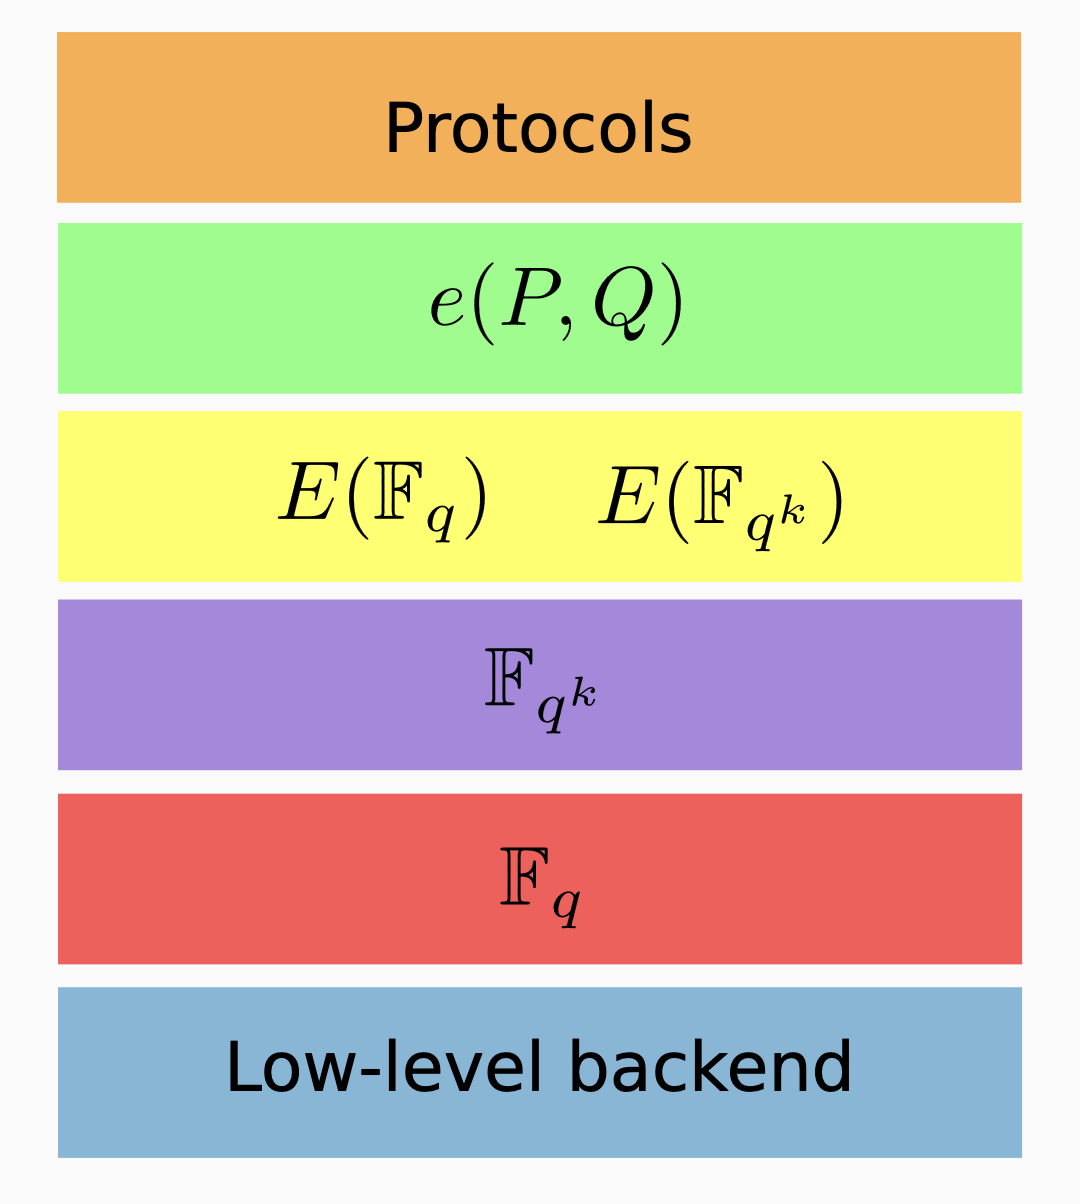
\includegraphics[width=0.5\textwidth]{images/levels.png}
            \caption{Various things under the hood.}
        \end{figure}
    \end{frame}
    \subsubsection{Field Extensions}
    \begin{frame}{What are field extensions?}
        These are ``like'' complex numbers $\mathbb{C}$. Recall that the complex number is $a+ib$ where $a,b \in \mathbb{R}$ and $i^2=-1$. So that:
        \begin{gather*}
            (a+ib)(c+id) = ac+(ad)i+(bc)i+(bd)i^2 \\
            = (ac-bd) + (ad+bc)i
        \end{gather*}
        \pause
        \textbf{Field extension} $\mathbb{F}_{p^2}$ is $a+ib$ where $a,b \in \mathbb{F}_p$ and $i^2=-1$. The same structure, essentially :)
        \pause
        
        Problems happen with $\mathbb{F}_{p^{6}}$ and $\mathbb{F}_{p^{12}}$ though since the intuition with complex numbers break...
    \end{frame}

    \begin{frame}{Polynomials}
        \begin{block}{Definition}
        \textbf{Polynomial} $K[X]$ is an expression
        \begin{equation*}
            p(X) = c_0 + c_1X + c_2X^2 + \dots + c_nX^n, \; c_i \in K
        \end{equation*}
        \end{block}
        \pause
        \begin{block}{Definition}
        Polynomial $p \in K[X]$ is said to be irreducible if there are two non-constant polynomials $q, r \in K[X]$ such that $p=qr$. 
             
        \textbf{Example:} $X^2+4 \in \mathbb{R}[X]$ is irreducible.
        \end{block}
        \pause   
        \begin{block}{Definition}
            \textbf{Quotient group} $K[X]/\langle p\rangle$ (which is a field) over irreducible polynomial $p$ is polynomials from $K[X]$ modulo $p$.
        \end{block}
    \end{frame}

    \begin{frame}{Examples}
        \begin{exampleblock}{Arithmetic in quotient group}
            Suppose $K=\mathbb{R}$ and $p(X)=X^2+1$ -- irreducible over $\mathbb{R}$. Then, example elements are $1+2X,2+3X \in \mathbb{R}[X]/\langle X^2+1 \rangle$. You can do the regular arithmetic with them:\pause
            \begin{itemize}
                \item \textbf{Addition:} $(1+2X)+(2+3X)=3+5X$ \pause
                \item \textbf{Multiplication:} $(1+2X)(2+3X)=2+7X+6X^2$. But, we need to reduce $\text{mod} \; (X^2+1)$. So notice that
                \begin{equation*}
                    6X^2+7X+2 \pause = 6(X^2+1) + \underbrace{(-4+7X)}_{\text{result}}
                \end{equation*}
                \item \pause Division (except for by $0+0X$) and subtraction is also allowed.
            \end{itemize}
        \end{exampleblock}
    \end{frame}

    \begin{frame}{Analogy!}
        In fact, $\mathbb{R}[X]/(X^2+1)$ is the same structure as complex numbers! (Formally, they are isomorphic $\mathbb{R}[X]/\langle X^2+1 \rangle \cong \mathbb{C}$). For example, when we multiplied $(1+2X)(2+3X)$, we got $-4+7X$. But...
        \begin{equation*}
            (1+2i)(2+3i) = 2 + 7i + \underbrace{6i^2}_{=-6} = -4 + 7i
        \end{equation*}
        
        \pause
        \vspace{10px}
        Notice, that $\mathbb{R}[X]/(X^2+9)$ would have a similar structure and is also isomorphic to $\mathbb{C}$. Thus, the choice of $p(X)$ is \textbf{not unique}.
    \end{frame}

    \begin{frame}{Tower of Extensions}
        We are ready to define $\mathbb{F}_{p^{12}}$. So,

        \begin{block}{Tower of Extensions}
        To define $\mathbb{F}_{p^{12}}$, we use the following objects with $\beta=-1 \in \mathbb{F}_p,\xi=9+u \in \mathbb{F}_{p^2}$:
        \begin{gather*}
            \mathbb{F}_{p^2} = \mathbb{F}_p[u] / \langle u^2 - \beta \rangle \\
            \mathbb{F}_{p^6} = \mathbb{F}_{p^2}[v] / \langle v^3 - \xi\rangle \\
            \mathbb{F}_{p^{12}} = \mathbb{F}_{p^6}[w] / \langle w^2 - v\rangle
        \end{gather*}
        \end{block}
    \end{frame}

    \begin{frame}{Visualization (sort of)}
       \begin{figure}
        \centering
        \includegraphics[width=0.7\textwidth]{images/tower.pdf}
        \caption{Tower of extensions visualized}
    \end{figure} 
    \end{frame}

    \begin{frame}{Formulating more simply}
        More simply:
        \begin{itemize}
            \item $\mathbb{F}_{p^2}$ is a number $a+bu$ where $a,b\in\mathbb{F}_p$ and $u^2=-1$.
            \item $\mathbb{F}_{p^6}$ is a number $a+bv+cv^2$ where $a,b,c \in \mathbb{F}_{p^2}$ and $v^3 = 9+u$.
            \item $\mathbb{F}_{p^{12}}$ is a number $a+bw$ where $a,b \in \mathbb{F}_{p^6}$ and $w^2=v$.\pause
        \end{itemize}

        \begin{exampleblock}{Intuition}
            You should regard an element from $\mathbb{F}_{p^k}$ as a regular number, but composed of $k$ scalars from $\mathbb{F}_p$ in a ``special'' way.
        \end{exampleblock}
    \end{frame}

    \subsubsection{Twisted Curve}

    \begin{frame}{Curves used}
        As mentioned, $\mathbb{G}_1$ is a regular curve $y^2 = x^3+3$.
        
        However, $\mathbb{G}_2$ is a curve (called \textbf{twisted curve}):
        \begin{equation*}
            y^2 = x^3 + \frac{3}{9+u}, \; \text{where}\; x,y \in \mathbb{F}_{p^2}
        \end{equation*}

        \pause So the element in $\mathbb{G}_2$ is described using four scalars from $\mathbb{F}_p$:
        \begin{equation*}
            (a+bu, c+du), \;\; a,b,c,d \in \mathbb{F}_p
        \end{equation*}

        \pause To conclude:
        \begin{itemize}
            \item $\mathbb{G}_1$ is a group of points on the curve $y^2=x^3+3$ over $\mathbb{F}_p$.
            \item $\mathbb{G}_2$ is a group of points on the curve $y^2=x^3+\frac{3}{9+u}$ over the field extension $\mathbb{F}_{p^2}$.
            \item $\mathbb{G}_T \text{\;``=''\;} \mathbb{F}_{p^{12}}^{\star}$ is a multiplicative subgroup of scalars from $\mathbb{F}_{p^{12}}$.
        \end{itemize}
    \end{frame}
    
    \begin{frame}{What it takes to implement?}
        \begin{block}{Calculating pairing $e(P,Q)$}
        \begin{enumerate}
            \item $x \gets \mathsf{MillerLoop}(P,Q) \in \mathbb{F}_{p^{12}}$.
            \item $f \gets \mathsf{FinalExp}(x) = x^{(p^{12}-1)/q} \in \mathbb{F}_{p^{12}}$.
            \item \textbf{return} $f$.
        \end{enumerate}
        \end{block}

        So, one needs to:
        \begin{enumerate}
            \item Implement $\mathsf{MillerLoop}$ that outputs the scalar $f$ in $\mathbb{F}_{p^{12}}$, also called a \textit{Tate pairing}.\pause
            \item Implement final exponentiation (\textsf{FinalExp}) that raises $f$ to the power of $(p^{12}-1)/q$ -- this ensures there are no equivalence classes in the output (called \textit{Reduced Tate pairing} or simply \textit{ate pairing}).\pause
        \end{enumerate}

        Again, understanding the construction requires ton of theory (in particular, from abstract geometry), but the algorithms are quite concrete.
    \end{frame}

    \begin{frame}{Some excerpts from papers...}
        \begin{figure}
            \centering
            \includegraphics[width=\textwidth]{images/miller.png}
            \caption{Miller Loop algorithm formalized.}
        \end{figure}
    \end{frame}

    \begin{frame}{Some excerpts from papers...}
        \begin{figure}
            \centering
            \includegraphics[width=0.5\textwidth]{images/finalexp.png}
            \caption{Final Exponentiation formalized.}
        \end{figure}
    \end{frame}

    \begin{frame}{So many are still uncovered...}
        \begin{enumerate}
            \item Useful curve endomorphisms (Kobitz curves) for $\boldsymbol{\mathsf{ecmul}}$.
            \item GLV decomposition.
            \item Arithmetics over NonNativeFields.
            \item Divisors and line function evaluations.
            \item Embedding degree and what $r$-torsion subgroups are.
            \item Torus $\mathbb{T}_2$ compression.
            \item ...
        \end{enumerate}
    \end{frame}
    
	\begin{frame}{}
      \centering \Large
      \emph{Thanks for your attention!}
    \end{frame}
\end{document}